\documentclass[12pt]{article}%
\usepackage{amsmath,amssymb,amsthm,amsfonts}
\usepackage{wasysym}
\usepackage{graphicx}
% \usepackage[poorman]{cleveref}
\usepackage{hyperref}
\usepackage[dvipsnames]{xcolor}
\usepackage{stackengine}
\usepackage[english]{babel}
\def\stackalignment{l}
% \usepackage[colorlinks]{hyperref}
\usepackage{tikz}
\usepackage[export]{adjustbox}
\usepackage{commands}

%\usepackage{geometry}
%\geometry{top = 0.9in}
\usepackage{appendix}

% \newcounter{subfigure}
\theoremstyle{plain}
\newtheorem{lemma}{Lemma}
\newtheorem{theorem}{Theorem}

\definecolor{red}{rgb}{0.8500, 0.3250, 0.0980}
\definecolor{green}{rgb}{0.4660, 0.6740, 0.1880}
\definecolor{yellow}{rgb}{0.9290, 0.6940, 0.1250}
\definecolor{blue}{rgb}{0, 0.4470, 0.7410}


\begin{document}

\title{Distributional Sparsity of Kantorovich Solutions}

\author{Stefan Steinerberger and Alex Johnson}
\date{\today}

\maketitle


% \begin{abstract}

% \end{abstract}


\section{Writeup of results so far}
\label{Sec: Intro}
In our project, we consider two sets of finite points $X,Y$ where $\abs{X} = m$ and $\abs{Y} = n$ and $m \neq n$ necessarily. Further we look at the empirical measures
\begin{align}\label{eq:empmeas}
  \mu = \frac{1}{m}\sum_{i=1}^{m}\delta_{x_i} ~~\text{and}~~ \nu = \frac{1}{n}\sum_{j=1}^{n}\delta_{y_j}
\end{align}
to motivate the problem of optimally transporting the mass from $X$ to $Y$. The case when $m=n$ is well studied, as Birkhoff's theorem implies that there is a transport plan bijection $\pi: X \to Y$ that permutes indices in $Y$ such that $\pi$ is optimal according to the Kantorovich problem. Recently, Steinerberger and Hosseini proved the following theorem:
\begin{theorem}
  Let $\mu$ and $\nu$ be defined as in \ref{eq:empmeas}. Then there is a solution of the Kantorovich problem such that mass from each point in $X$ is moved to at most $\frac{n}{\mathrm{gcd}(m,n)}$ different points in $Y$ and that each point in $Y$ receives mass from at most $\frac{m}{\mathrm{gcd}(m,n)}$ points in $X$.
\end{theorem}
In building off of this work and this theorem, we investigate the problem of knowing the distributions of the number of different points moved from $X$ to $Y$, and vice-versa, as $\frac{n}{\mathrm{gcd}(m,n)}$ and $\frac{m}{\mathrm{gcd}(m,n)}$ may be large. As an example, if $m=20$ and $n=30$, then we know that each point in $X$ is mapped to at most 3 points in $Y$, and each point in $Y$ receives mass from at most $2$ points in $X$. Yet, we seek to understand the frequency with which a point in $X$ is mapped to at most 3 points in $Y$, for instance. On simple intuition, we know that this exact scenario shouldn't happen which relatively high frequency, since points will optimally be matched to those points closest to them (on average). We investigate this question both numerically and theoretically. Specifically numerically, we look at specific interesting cases, such as when $m,n$ are two (relatively) large, coprime numbers, and when $m,n$ are again coprime but with large distance from each other. To our surprise, we found that the distribution of points tends to have small support, consistently grouping across a small number of points that are always close together.

Let's take a look at a couple more in-depth examples of what was motivated above. First, let's look at the distribution created by matching $m=57$ points in $X$ to $n=79$ points in $Y$. Note, clearly, $m,n$ are coprime. This distribution is shown in \ref{fig: A}.
\begin{figure}
  \centering
  \hspace*{0cm}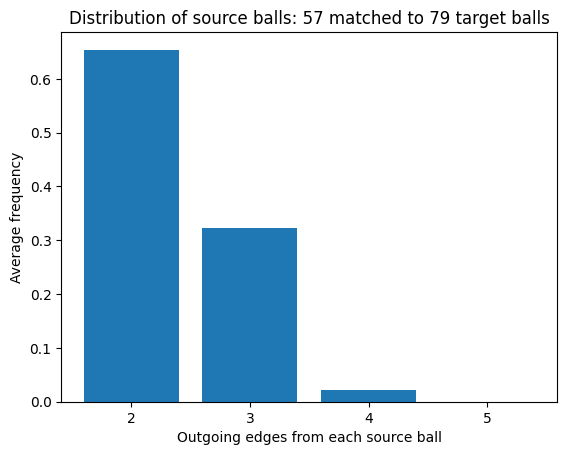
\includegraphics[width=1\textwidth,height=\textwidth,keepaspectratio]{images/57-79.png}
  \caption{}
  \label{fig: A}
\end{figure}

% \section{Theoretical Background}



% \section{Numerical Methods}

% \section{Conclusion}\label{Sec: Conclusion}


% \section*{Acknowledgment}





\end{document}
